The interaction of light with any other object is described best with a set of 
equations called the Maxwell equations. This set of equations fully capture and 
describes the electromagnetic wave nature of light. It relates point wise the 
electric wave vector $\vb{E}$, the magnetic induction $\vb{B}$, the electric 
current density $\vb{j}$, the electric displacement $\vb{D}$, and the magnetic 
vector $\vb{H}$ with each other for objects where the physical properties are 
continuous in the neighbourhood of the point of interest~\cite{Born1980Ch1}
\begin{subequations}
  \begin{align}
    \curl{\vb{H}} - \frac{1}{c}\pdv{t}\vb{D} &=\frac{4\pi}{c}\vb{j} 
    \label{eq:Th-ampere} \\
    \curl{\vb{E}} - \frac{1}{c}\pdv{t}\vb{B} &=  0
    \label{eq:Th-faraday} \\
    \div{\vb{D}} &= 4\pi\rho_{\MR{E}}
    \label{eq:Th-gauss} \\
    \div{\vb{B}} &= 0
    \label{eq:Th-gauss-mag}
  \end{align}
\end{subequations}
with $c$ being the speed of light and $\rho_{\MR{E}}$ the total electric charge 
density. Although, 
\cref{eq:Th-ampere,eq:Th-faraday,eq:Th-gauss,eq:Th-gauss-mag} describe the 
behavior of light fully, it is often more convenient to think of light as a 
collection of single rays. In the limit of a vanishing small light wavelengths 
$\lambda_{\text{light}}$ compared to the object size $R$, the approximation of 
light as single rays is valid~\cite{Born1980Ch3}. This branch of describing the 
propagation of light is called -- amongst others -- \emph{Ray Optics}.

Our laser has a wavelength of $\lal=\SI{785}{\nm}$ and the smallest object we 
use has a radius of $R=\SI{1.03}{\um}$. The ratio $\sfrac{2R}{\lal}\approx 2.6$ 
is close to unity and the application of ray optics in our case might be 
questionable. However, previous works with our optical trap
\cite{Lakaemper2015,Lamprecht2016,Lamprecht2017} have shown that the ray 
approximation is a reasonable approach in our case. In addition, one has to 
differentiate between quantitative and qualitative analysis. In all here 
presented results we use our optical trapping setup as tool for relating 
results qualitatively.

\section{Experimental Setup}

\begin{figure}[tbp]
  \centering
  % \tikzsetnextfilename{setup}

  \definecolor{tempcolor}{RGB}{176, 206, 255}
\pgfmathdeclarefunction{gauss}{2}{%
  \pgfmathparse{1/(#2*sqrt(2*pi))*exp(-((x-#1)^2)/(2*#2^2))}%
}

\begin{tikzpicture}

  \shade[top color=white,bottom color=white,middle color=red] (3,-0.15) 
  rectangle ++(2.5,0.3);

  \shade[top color=white,bottom color=white,middle color=red] (5.5,-1.25) 
  rectangle (10,1.25);

  % laser head
  \filldraw[color=black,fill=black!50] (0,-0.5) rectangle ++(3,1);
  \node at (1.5,0) {Laser head};

  % lens
  \fill[tempcolor] (5.5,0) ellipse (0.15 and 1.5);
  \path (5,1.5) -- ++(1,0) node[above, midway, anchor=south] {Expanding lens};

  % microscope
  \filldraw[white] (9,-2) rectangle ++ (2,4);
  \filldraw[black] (9,-0.2) rectangle (9.2,-1.5);
  \filldraw[black] (9,0.2) rectangle (9.2,1.5);
  \filldraw[red] (9,-0.2) rectangle ++(1.5,0.4);

  \draw[black,thick] (10,-1) -- ++(0,0.8) -- ++(0.3,0) -- ++(0,0.4) -- 
  ++(-0.3,0) -- ++(0,0.8);

  \path (7.0,1.5) -- ++(4,0) node[above, midway, anchor=south, align=center] 
  {Microscope housing};

  \draw[black, very thick, ->] (11,0) -- ++(1.5, 0) -- ++(0, -4) -- ++(-1.5,0);

  \draw[black!70, thin] (7,-0.21) -- ++(2,0);
  \draw[black!70, thin] (7,+0.21) -- ++(2,0);

  %% bottom
  \fill[tempcolor] (10,-4) ellipse (0.15 and 0.75);
  \path (9.5,-3.25) -- ++(1,0) node[above, midway, anchor=south] {Focussing 
  lens};

  \coordinate (M) at (8.5,-4);
  \draw[black,thin,->] (M) -- node[above,pos=0.9] {\tiny$\ex$} ++(0,0.5);
  \draw[black,thin,->] (M) -- node[above,pos=0.9] {\tiny$\ey$} ++(0.4,0.4);
  \draw[black,thin,->] (M) -- node[above,pos=0.9] {\tiny$\ez$} ++(-0.5,0);
  \shade[ball color=black!10] (M) circle (.25);

  \path (8.25,-4.5) -- ++(0.5,0) node[below, midway] {particle};

  \fill[tempcolor] (7.0,-4) ellipse (0.15 and 0.75);
  \path (6.5,-3.25) -- ++(1,0) node[above, midway, anchor=south] {Condensor 
  lens};

  \filldraw[color=black, fill=black!50] (5.8,-4.5) rectangle ++(-1,1);
  \path (4.8,-4.5) -- ++(1,0) node[below, midway, anchor=north] {Filter};

  \fill[tempcolor] (2.5,-4) ellipse (0.15 and 0.75);
  \path (2,-3.25) -- ++(1,0) node[above, midway, anchor=south] {Lens 3};

  \filldraw[color=black, fill=black!10] (0,-4.4) rectangle ++(0.8,0.8);
  \draw[thick,black,dotted] (0,-4) -- ++(0.8,0);
  \draw[thick,black,dotted] (0.4,-4.4) -- ++(0,0.8);

  \path (0,-3.5) -- ++(0.8,0) node[above, midway, anchor=south] {QPDxy};
  \filldraw[color=red!50] (0.4,-4) circle (.2);

  \draw[red, thick] (11, -3.6) -- ++(-1,0) -- ++(-3,-0.8) -- (5.8,-4.4);
  \draw[red, thick] (11, -4.4) -- ++(-1,0) -- ++(-3,+0.8) -- (5.8,-3.6);
  \draw[red!50, thick, dashed]  (4.8,-4.4) -- (2.5,-4.4) -- (0.4,-3.8);
  \draw[red!50, thick, dashed]  (4.8,-3.6) -- (2.5,-3.6) -- (0.4,-4.2);

  % beam splitter
  \draw[gray,very thick] (3.2,-3.5) -- ++(1,-1);
  \path (3.2,-4.5) -- ++(1,0) node[below,midway] {Splitter};

  \fill[tempcolor] (3.7,-2.5) ellipse (0.75 and 0.15);
  \path (4.6,-2.5) -- ++(1,0) node[midway] {Lens 4};

  \filldraw[color=black, fill=black!10] (3.3,-2.0) rectangle ++(0.8,0.8);
  \draw[thick,black,dotted] (3.7,-2) -- ++(0,0.8);
  \draw[thick,black,dotted] (3.3,-1.6) -- ++(0.8,0);
  \path (2.9,-1.6) -- ++(-0.8,0) node[midway] {QPDz};

  \filldraw[color=red!50,opacity=0.3] (3.7,-1.6) circle (0.6);

  \draw[red!50, thick, dashed]  (3.3,-3.6) -- ++(0,1.1) -- (4.3,-2);
  \draw[red!50, thick, dashed]  (4.1,-4.4) -- ++(0,1.9) -- (3.1,-2);


\begin{axis}[
    domain=-0.15:0.15,
    samples=200,
    no markers,
    axis lines=none,
    ticks=none,
    xmin=-1,
    xmax=1,
    ymax=250,
    anchor = origin,
    rotate around={270:(current axis.origin)},
    hide axis,
    yshift=36mm
    ]

    \addplot[black] {gauss(0,0.01)};

\end{axis}

\begin{axis}[
    domain=-0.3:0.3,
    samples=100,
    no markers,
    axis lines=none,
    ticks=none,
    xmin=-1,
    xmax=1,
    ymax=20,
    anchor = origin,
    rotate around={270:(current axis.origin)},
    hide axis,
    yshift=65mm
    ]

    \addplot[black] {gauss(0,0.15)};

\end{axis}

\end{tikzpicture}

  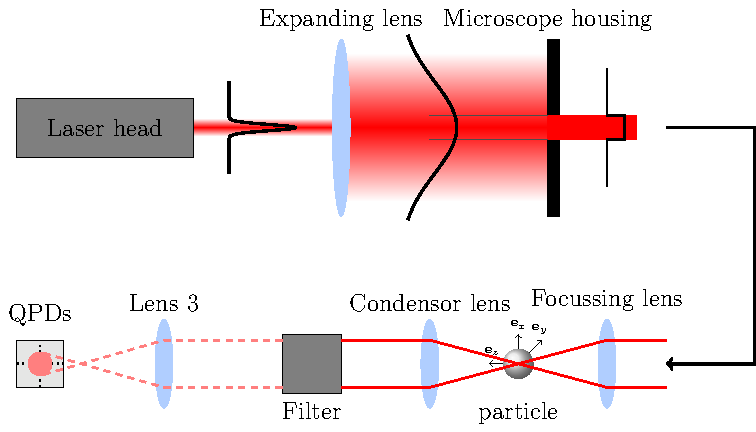
\includegraphics[]{Plots/cache/setup.pdf}
  \caption{Schematic of light path from laser head to quadrant photo detectors. 
  In the top half sketch red shading and the black lines the laser intensity 
profile qualitatively. In the bottom half just the outer most laser rays are 
depicted.}
  \label{fig:Th-setup}
\end{figure}

Before highlighting important parts from ray optics it is advantageous to 
understand our optical trapping setup which is based upon the work of Arthur 
Ashkin~\cite{Ashkin1978,Ashkin1987,Ashkin2002,Ashkin1986,Ashkin1992,Ashkin1997}. 
\cref{fig:Th-setup} depicts a basic schematic of the laser path from the laser 
source to the quadrant photo detectors (QPDs) in the back focal plane. A 
complete overview of our setup with a list and explanation of every used part 
is available in~\cite{Lamprecht2017}.

Our laser diode emits a tightly confined laser beam in the near-infrared regime 
(non-visible) with a wavelength of $\lal=\SI{785}{\nm}$ and a maximal power of 
$P=\SI{200}{\milli\watt}$ and with a transverse electromagnetic mode of order 
00 (TEM$_{00}$). This laser profile is axisymmetric to the light propagation 
direction and can be visualized with a rotating Gaussian bell curve. Next, the 
beam is expanded such that it is much larger than the opening of the microscope 
housing. The magnitude of the trapping forces are proportional to the laser 
intensity of the beam. The biggest contribution to the total force stems from 
the outer parts of the beam. Therefore, it is advantageous to broaden the beam 
before guiding it to the focusing lens. The opening of the microscope is 
overfilled by the broadened beam and the laser intensity after this cutoff can 
be approximated with a flat-top profile. Hence, every light wave (also the ones 
contributing most to the total trapping force) carries the same intensity.

The next step is the focusing of the beam with a high numerical aperture (NA) 
oil immersion lens. Here, the actual trapping of the particle occurs. If more 
than just the trapping of particles is of interest, the beam needs to be 
investigated further. The relative movement of the particle within the trap 
contains the necessary information. In order to image the movement in the $\ex$ 
and $\ey$ direction the beam is collimated again by the condensor lens after it 
passed the particle and filtered to reduce its total intensity to prevent 
damage of the QPDs. Before the beam is focussed, it is split into two because 
the axial movement detection for $\ez$ and the in plane movement detection for 
$\ex$ and $\ey$ have inherently different working principles.

If the particle moves within the trap the spot on the QPDxy will also move. By 
measuring the voltage on each quadrant of the QPDxy and summing and subtracting 
certain quadrants it is possible to retrieve the information about the movement 
in each direction separately. For the axial direction the opening of the QPDz 
is overfilled. An axial movement of the particle causes a change of total 
intensity on this QPD. By measuring the QPDz total intensity we have the 
information about the relative movement of the particle within the trap. After 
the calibration of the OT the measured voltages that are proportional to the 
particle movement can be converted to the physical unit meter. The calibration 
process itself is not relevant for this thesis but is available 
here~\cite{Lamprecht2017}. An discussion of different calibration options is 
available from \citeauthor{Svoboda1994}~\cite{Svoboda1994} and 
\citeauthor{Jun2004}~\cite{Jun2004}.


\textcolor{red}{which material parameters if fluid or water}

\section{Ray Optics\label{sec:Th-rayoptics}}

As said before, in the regime of ray optics the propagation of light is 
visualized by single rays. The interaction of a single ray at an interface is 
then studied geometrically. The defining property for these kind of 
investigations is the so called refractive index $\refraction$. Light travels 
in vacuum at speed of light $c=\SI{299792458}{\m\per\s}$. In other mediums than 
vacuum the speed of light has a different (smaller) magnitude. The refractive 
index relates the speed of light of vacuum $c$ to any other material $c_{\Box}$
\begin{equation}
  c_{\Box} = \frac{c}{n}.
  \label{eq:Th-lightspeed}
\end{equation}
Since there is nothing faster than the speed of light, the refractive index 
$\refraction$ cannot be smaller than 1. This index is not constant for one 
material but a function of the wavelength $\lambda$. Additionally, the 
refractive is in general a complex quantity
\begin{equation}
  \refraction\geq 1 \quad \wedge \quad \refraction \coloneqq 
  \refraction(\lambda) = \refraction(\lambda) - \iu k(\lambda)
  \label{eq:Th-refractive-index}
\end{equation}
where $k$ is called the extinction coefficient~\cite{Jackson2013}. 
\Cref{fig:Th-n_water} depicts $n$ and $k$ of water for different wavelengths 
$\lambda$. Whereas the real part of \cref{eq:Th-refractive-index} is about 
constant for $\lambda > \SI{400}{\nm}$, the complex part changes its magnitude 
over 4 orders of magnitude in the same interval.

\begin{figure}[tbp]
  \centering
  % \tikzsetnextfilename{n_water}
%%%%%%%
% READ TABLE
%%%%%%%

\begin{tikzpicture}
\begin{axis}[
  height=80mm,
  width=120mm,
  no markers,
  xlabel={$\lal$ [\si{\nm}]},
  ylabel={$\nreal$ [-]},
 ]

    \addplot[black] table[x=wl,y=n] 
    {\relPath/10_Figures/TikZ/Segelstein1981a.dat};

    \label{plot_n}
    \draw[dashed,<->,latex-latex] ({axis cs:785,0}|-{rel axis cs:0,0.0}) -- 
    (785,1.326244) -- node[above,pos=0.65,fill=white,opacity=0.8,text 
    opacity=1] {\footnotesize 1.326} ({0,1.326244}-|{rel axis cs:0,0});
\end{axis}
\begin{axis}[
  height=80mm,
  width=120mm,
  axis y line*=right,
  axis x line=none,
  ylabel={$\alpha$ [\si{\per\meter}]},
  no markers,
  ymode = log,
]
    \addlegendimage{/pgfplots/refstyle=plot_n}\addlegendentry{$\nreal$}
    \addplot[black,dash dot] table[x=wl,y=a] 
    {\relPath/10_Figures/TikZ/Segelstein1981a.dat};
    \addlegendentry{$\alpha$}

    \draw[dashed,<->,latex-latex] ({axis cs:785,0}|-{rel axis cs:0,0.0}) -- 
    (785,2.144) -- node[above,pos=0.73] {\footnotesize 2.144} 
    ({0,2.144}-|{rel axis cs:1,0});
    % 2.14353e+00

    \draw[dotted,<->,latex-latex] ({axis cs:1060,0}|-{rel axis cs:0,0.0}) -- 
    (1060,15.40) -- node[above,pos=0.53,fill=white,opacity=0.8,text 
    opacity=1] {\footnotesize 15.40} ({0,15.40}-|{rel axis cs:1,0});
    % 1.53991e+01
\end{axis}
\end{tikzpicture}

  \includegraphics[]{Plots/cache/n_water.eps}
  \caption{Index of refraction $n$ and extinction coefficient $k$ for water 
  over wavelength $\lambda$. Data taken from \cite{Hale1973,Segelstein1981}.}
  \label{fig:Th-n_water}
\end{figure}


The absorption coefficient~\cite{Hecht2017}
\begin{equation}
  \alpha = \frac{4\pi f k}{c} = \frac{4\pi}{\lambda}k
  \label{eq:Th-alpha}
\end{equation}
converts the dimensionless quantity $k$ into a physical parameter with unit 
\si{\per\meter}. Any ray of any wavelength is attenuated when propagating 
through a medium. The \emph{Beer-Lambert Law}
\begin{equation}
  \intensity(s) = \intensity_{0}\exp(-\alpha s)
  \label{eq:Th-beer-lambert}
\end{equation}
captures the change of intensity while moving along the path $s$ where 
$\intensity_{0}$ is the intensity at the start. E.g. in a depth of 
approximately \SI{1}{\kilo\meter} it is completely dark in the ocean because 
all the intensity of the sunlight is attenuated there.

\begin{figure}[tbp]
  \centering
  % \tikzsetnextfilename{Snell}

\tikzstyle arrowstyle=[scale=1]

\tikzstyle directed=[postaction={decorate,decoration={markings,
    mark=at position .65 with {\arrow[arrowstyle]{stealth}}}}]

\tikzstyle reverse directed=[postaction={decorate,decoration={markings,
    mark=at position .65 with {\arrowreversed[arrowstyle]{stealth};}}}]

\tikzset{SnellNode/.style={text width=10mm, align=center}}

\begin{tikzpicture}
  \def\W{5}
  \def\H{4}
  \def\x{0.95}
  \def\anglealpha{0}
  \pgfmathsetmacro{\y}{{(1-\x)*\H}}
  \pgfmathsetmacro{\radius}{(\W^2+\y^2)/2/\y}
  \pgfmathsetmacro{\anglealpha}{{asin(\W/\radius)}}
  \pgfmathsetmacro{\s}{{90+\anglealpha}}
  \pgfmathsetmacro{\e}{{90-\anglealpha}}

  \pgfmathsetmacro{\anglebeta}{{0.8*\anglealpha}}
  \pgfmathsetmacro{\p}{{(\radius-\H)*sin(\anglebeta)}}
  \pgfmathsetmacro{\px}{{\radius*sin(\anglebeta)}}
  \pgfmathsetmacro{\py}{{-\radius*(1-cos(\anglebeta))}}


  % define coordinates
  \coordinate (O) at (0,0) ;
  \coordinate (A) at (0,\H) ;
  \coordinate (B) at (0,-\H) ;

  % media
  \fill[blue!20,opacity=.3] (-\W,0) rectangle (\W,\H);
  \fill[black!10!,opacity=.3] (-\W,0) rectangle (\W,-\H);
  \node[right, SnellNode] at (2,1.5) {{Fluid\\ $\nf$}};
  \node[left, SnellNode] at (-2,-2) {{Particle\\ $\ns$}};

  % axis
  \draw[dash pattern=on5pt off3pt] (A) -- (B) ;
  % normal
  \draw[|->, thick] (0,0) -- node[right, pos=1] {$\normalvector$} (0, 2.5);


  % ray representation
  \def\gamma{130}
  \draw[red, variable=\x, domain=2.5:\W, samples=100] (0,\H) plot 
  ({\x*cos(\gamma)-cos(\x*pi r*3)/4*sin(\gamma)},{sin(\gamma)*\x+cos(\x*pi 
  r*3)/4*cos(\gamma)});

  % rays
  \draw[red,ultra thick,reverse directed] (O) -- node[left, xshift=-1mm, 
  pos=0.2] {$P_{\mathrm{i}}$} (130:5.2);

  \draw[red,ultra thick,directed] (O) -- node[right, xshift=1mm, pos=0.2] 
  {$P_{\mathrm{r}}$} (50:5.2);

  \draw[blue,directed,ultra thick] (O) -- node[right, xshift=1mm, pos=0.2] 
  {$P_{\mathrm{t}}$} (-70:4.24);

  % particle circumference
  \draw (-\W,-\y) arc (\s:\e:\radius);
  \draw[black,->|,>=stealth'] (\p,-\H) -- node[right, pos=0.7] {$\R$} (\px, 
  \py);

  % angles
  \draw[->,>=stealth'] (0,1) arc (90:130:1);
  \draw[->,>=stealth'] (0,1) arc (90:50:1);
  \draw[->,>=stealth'] (0,-1.4) arc (270:290:1.4);

  \node[] at (280:1.8)  {$\transmitted$};
  \node[] at (110:1.4)  {$\incident$};
  \node[] at (70:1.4)  {$\refracted$};

\end{tikzpicture}

  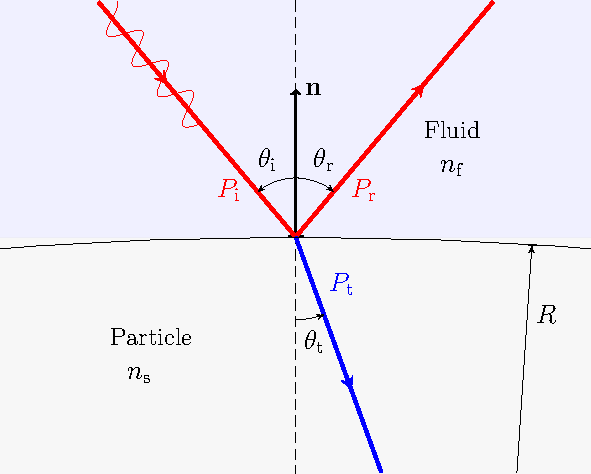
\includegraphics[]{Plots/cache/Snell.pdf}
  \caption{Visualization of \emph{Snell's Law} for rays at an interface of two 
  media with different refractive indices $\refraction_{\Box}$.}
  \label{fig:Th-Snell}
\end{figure}

With the real part of the complex refractive index, it is possible to define 
the most important relation in the ray optics regime. The \emph{Snell's Law} 
(see also \cref{fig:Th-Snell}) is defined as
\begin{equation}
  \nf\,\sin\incident = \ns\,\sin\transmitted.
  \label{eq:Th-Snell}
\end{equation}
It connects the angle of incident $\incident$ with the transmitted angle 
$\transmitted$ at an interface of two different media with refractive indices 
$\ns$ and $\nf$, respectively. This law is based on the fact that a ray of 
light travels on the fastest path (not the shortest) between two 
points~\cite{Born1980Ch3}. The angle of the reflected ray is equal to the 
incident angle ($\reflected=\incident$).

There is one more angle of special interest. It is the angle of total internal 
reflection $\theta_{\MR{TIR}}$
\begin{equation}
  \theta_{\MR{TIR}}=\incident \quad\forall\quad \frac{\nf}{\ns}\,\sin\incident 
  > 1.
  \label{eq:Th-TIR}
\end{equation}
For incident angles of this magnitude or greater 
($\incident\geq\theta_{\MR{TIR}}$), no ray is transmitted into the other 
medium. This can only occur if the index of refraction of the incident medium 
is greater than the transmitted medium ($\nf>\ns$ in \cref{fig:Th-Snell}) 
otherwise the ratio $\sfrac{\nf}{\ns}$ of \cref{eq:Th-TIR} is always smaller 
than unity and there is physically no total internal reflection possible.

% The other angle of special interest is the so called \emph{Brewster Angle} 
% $\theta_{\MR{B}}$
% \begin{equation}
  % \theta_{\MR{B}} = \tan^{-1}\left( \frac{\ns}{\nf} \right).
  % \label{eq:Th-brewster}
% \end{equation}
% At this angle there does not occur an reflection and hence all the intensity is 
% transmitted.

So far, \cref{eq:Th-Snell} calculates in which direction a ray will travel 
after an interface of two media. The amplitude of the reflected and transmitted 
rays can be computed with the so called \emph{Fresnel 
Equations}~\cite{Jackson2013,Born1980Ch1}. Although we think of light as rays, 
the theory behind those equations is based on the electromagnetic wave 
character of light. For time harmonic electromagnetic waves the amplitude of 
the incident electric wave vector $\vb{E}_{\MR{i}}$ to the transmitted 
$\vb{E}_{\MR{t}}$ and to the reflected $\vb{E}_{\MR{t}}$ electric wave vector 
is related by $\fresnelr_{i}$ and $\fresnelt_{i}$
\begin{subequations}
\begin{align}
  \vb{E}_{\MR{r}} & =\fresnelr_{i}\,\vb{E}_{\MR{i}} \\[3mm]
  \vb{E}_{\MR{t}} & =\fresnelt_{i}\,\vb{E}_{\MR{i}}
\end{align}
\end{subequations}
where the subscript $i$ can either be $i=\MR{p}$ for p-polarized light or 
$i=\MR{s}$ for s-polarized light~\cite{Jackson2013,Born1980Ch1}. ``s'' and 
``p'' stand for the German words ``parallel'' (parallel) and ``senkrecht'' 
(perpendicular), respectively. They refer to the to the orientation of the 
incident electric field $\vb{E}_{\MR{i}}$ to the plane of incident. For the 
special cases of ``p'' and ``s'' polarized light the Fresnel coefficient with 
the assumption that both media are non-magnetic ($\mu_{\MR{f}} = \mu_{\MR{s}} = 
\mu_{0} = 1$)~\cite{Born1980Ch1} are
\begin{subequations}
\begin{align}
  \fresnelr_{\MR{s}} & =
  \frac{2\,\nf\,\cos\incident}{\nf\,\cos\incident + \ns\,\cos\reflected} 
  \label{eq:Th-fresnel-rs}\\[3mm]
  \fresnelt_{\MR{s}} & = \frac{\nf\,\cos\incident - 
  \ns\,\cos\reflected}{\nf\,\cos\incident + \ns\,\cos\reflected} 
  \label{eq:Th-fresnel-ts}\\[3mm]
  \fresnelr_{\MR{p}} & =
  \frac{2\,\nf\,\cos\incident}{\ns\,\cos\incident + \nf\,\cos\reflected} 
  \label{eq:Th-fresnel-rp}\\[3mm]
  \fresnelt_{\MR{p}} & = \frac{\ns\,\cos\incident - 
  \nf\,\cos\reflected}{\ns\,\cos\incident + \nf\,\cos\reflected}.
\label{eq:Th-fresnel-tp}
\end{align}
\end{subequations}
So far, the Fresnel coefficients relate the amplitudes of the incident 
electrical field to the transmitted and reflected electrical field. In general, 
the sum of $\fresnelr$ and $\fresnelt$ does not add up to unity.

For \cref{sec:Th-temperature}, it is necessary to know how much of the incident 
power $P_{\MR{i}}$ is transmitted and how much is reflected. The power 
$P=\intensity A$ is a product of the intensity $\intensity$ and the area $A$ it 
is acting on. The intensity is defined as the timeaverage of the Ponyting 
vector $\vb{S}$
\begin{equation}
  \intensity = \timeaverage{\abs{\vb{S}}} = 
  \timeaverage{\abs{\vb{E}_{0}\times\vb{H}_{0}}} = 
  \frac{1}{2}\,\frac{\refraction}{Z_{0}}\,\abs{\vb{E}_{0}}^{2} = 
  \frac{1}{2}\,\refraction\,c\epsilon_{0}\,\abs{\vb{E}_{0}}^{2}
\end{equation}
where $Z_{0}$ is the electrical impedance of free space and $\epsilon_{0}$ is 
the vacuum permittivity. With 
\cref{eq:Th-fresnel-rs,eq:Th-fresnel-ts,eq:Th-fresnel-rp,eq:Th-fresnel-tp} the 
scaling of the electrical field at the interface is defined. With the relation 
(see also \cref{fig:Th-Snell})
\begin{equation}
  w = \frac{w_{\MR{i}}}{\cos\incident} = \frac{w_{\MR{r}}}{\cos\reflected} = 
  \frac{w_{\MR{t}}}{\cos\transmitted}
  \label{eq:Th-area}
\end{equation}
and the scaling of the power
\begin{equation}
  P = \intensity A \propto \refraction\,\abs{\vb{E}_{0}}^{2}A \propto
  \refraction\,\abs{\vb{E}_{0}}^{2}w
\end{equation}
one can calculate the reflectance $\fresnelR_{i}$ as the ratio of the reflected 
power $P_{\MR{r}}$ to the incident power $P_{\MR{i}}$ as
\begin{equation}
  \fresnelR_{i} = \frac{P_{\MR{r}}}{P_{\MR{i}}} = 
  \frac{\intensity_{\MR{r}}\,\nf\,w_{\MR{r}}}{\intensity_{\MR{i}}\,\nf\,w_{\MR{i}}} 
  =\frac{\abs{\fresnelr_{i}\,\vb{E}_{0}}^{2}}{\abs{\vb{E}_{0}}^{2}} = 
  \fresnelr_{i}^{2}
  \label{eq:Th-fresnelR}
\end{equation}
where again the italic $i$ in the subscript ($\Box_{i}$) is the polarization. 
Similarly one finds the transmittance $\fresnelT_{i}$ as
\begin{equation}
  \fresnelT_{i} = \frac{P_{\MR{t}}}{P_{\MR{i}}} = 
  \frac{\intensity_{\MR{t}}\,\ns\,w_{\MR{t}}}{\intensity_{\MR{i}}\,\nf\,w_{\MR{i}}} 
  =\frac{\abs{\fresnelt_{i}\,\vb{E}_{0}}^{2}}{\abs{\vb{E}_{0}}^{2}}\,\frac{\ns\,w_{\MR{t}}}{\nf\,w_{\MR{i}}} 
  = \fresnelt_{i}^{2}\,\frac{\ns\,\cos\transmitted}{\nf\,\cos\incident}.
  \label{eq:Th-fresnelT}
\end{equation}
For unploarized rays one can take the arithmetic average of $\Box_{\MR{s}}$ and 
$\Box_{\MR{p}}$ polarization values. Other than the Fresnel coefficients the 
sum of the reflectance $\fresnelR$ and the transmittance $\fresnelT$ for one 
angle of incidence need to be unity
\begin{equation}
  \fresnelR + \fresnelT = 
  \frac{\fresnelR_{\MR{s}}+\fresnelR_{\MR{p}}}{2} +
  \frac{\fresnelT_{\MR{s}}+\fresnelT_{\MR{p}}}{2} = 1 
  \label{eq:Th-fresnel}
\end{equation}
because the incident power $P_{\MR{i}}$ is either reflected or transmitted
\begin{equation}
  P_{\MR{i}} = P_{\MR{r}} + P_{\MR{t}} = P_{\MR{i}}\left( \fresnelR + \fresnelT 
  \right).
\end{equation}

\section{Laser Induced Temperature Change\label{sec:Th-temperature}}

A laser is a (highly focused) coherent beam of electromagnetic waves of a 
single wavelength $\lal$. Intensities with the orders of 
\si{\mega\watt\per\square\meter} and more are common. For comparison, the 
average intensity of the sun on to the earth in Central Europe is about 
\SI{1.36}{\kilo\watt\per\square\meter}, and the laser of our setup has with its 
peak power of \SI{200}{\milli\watt} and a specified beam diameter of 
\SI{1}{\mm} a maximal intensity of about 
\SI{0.25}{\mega\watt\per\square\meter}. As described with the Beer-Lambert-Law
(\cref{eq:Th-beer-lambert}) some of the laser intensity is attenuated while 
traveling through any medium. The attenuation of intensity will lead to an 
increase of temperature in the absorbing medium.

The intensity of a focused laser is highest in the region of the focal point 
because all its power is confined to a small area. Direct temperature 
measurements in the vicinity of the laser focus are due to the microscopic 
region of interest up to now not possible. Precise knowledge of the temperature 
change is of interest, e.g., for the calibration process of the OT but also for 
objects that need to stay below a certain temperature, e.g. living cells.

In the following, we will first discuss the current research regarding 
temperature increase in OTs, discuss the path of a ray through the particle, 
and then motivate a temperature approximation based on simple ray optics.

\subsection{State of the Art}\label{sec:Th-state}

\cyear{Liu1995} measured the temperature dependent change in fluorescence of 
biological cells while being trapped with a wavelength of 
$\lal=\SI{1064}{\nm}$. They found a linear relation between temperature 
increase and applied laser power of about \SI{15}{\degreeCelsius\per\watt}. In 
addition, they solved the heat problem also analytically. For that, they 
neglected the trapped object and modeled as water because their cells of 
interest consist mainly out of water. The experiments as well as the 
analytical solution show an almost instantaneous change in temperature after 
the laser is switched on. \cyear{Celliers2000} measured the local change in the 
index of refraction for water while being subjected to a laser with a 
wavelength of \SI{985}{\nm}. During the measurements no objects was trapped in 
the laser focus. They measured a temperature increase of \SI{4}{\degreeCelsius} 
with a laser power of \SI{55}{\milli\watt} in the focus of the laser. An 
analytical model that utilized an improved source term compared to 
\cite{Liu1995} validated their results.

\cyear{Peterman2003} measured with a OT of \SI{1064}{\nm} wavelength the 
effects of the temperature increase in the vicinity of the laser focus. A 
change of temperature in the fluid will lead to a change of the fluid 
viscosity. The viscosity change alters the calibration parameters of the OT. By 
fitting the calibration parameters for different laser powers to the 
theoretical relation they found a temperature increase of roughly 
\SI{8}{\degreeCelsius\per\watt} for water as fluid medium and silica beads as 
trapped object. More interestingly, their analytical model revealed that most 
of the heat absorption is in the fluid rather than the trapped object. In 
addition, usual glass coverslips act as fast heat conductor compared to water 
such that measurements close to the top or bottom surface of the fluid cavity 
lead to a minor temperature increase.

\cyear{Moreau2015} injected Rhodamine B (RhB) in cells to measure the 
temperature change of an OT with \SI{800}{\nm} wavelength. RhB is a temperature 
sensitive dye which changes its fluorescence linearly with the temperature. 
Since they injected the RhB into the cell the measured temperature difference 
was around the focal point. As before, the increase of the temperature occurs 
almost instantaneously and is about \SI{9}{\degreeCelsius\per\watt}. Lastly, in 
\citeyear{Catala2017}, \cname{Catala2017} studied the effects of different 
experimental parameters (numerical aperture (NA), material of trapped object, 
distance to coverslips, object radius) to the magnitude of the temperature 
increase with an OT of \SI{1064}{\nm} wavelength. A numerical model validated 
their experimental findings. Their source term which is an extension to 
\cname{Peterman2003} takes account of the NA, the finite focal spot size, and 
the wavelength of the laser itself. In agreement to the others they found the 
heat increase to be about \SI{20}{\degreeCelsius\per\watt}.

All of the aforementioned studies (see also \cref{tab:Th-heating}) validated in 
their experiments the linear relation of the applied laser power to the 
increase in temperature. Also, they showed that the temperature change occurs 
almost instantaneously and that a steady system is established in the range of 
\si{\ms}. In addition, they agree that the main absorption occurs in the fluid 
medium (water or glycerol) rather than the trapped object (polystyrene or 
silica) itself because the absorption coefficient $\alpha$ is greater. However, 
as can be seen in \cref{fig:Th-n_water}, the extinction coefficient is 
dependent on the wavelength $\lal$. Besides \cite{Moreau2015} all studies 
operate at a wavelength of \SI{1064}{\nm}. Our OT operates at \SI{785}{\nm} and 
the extinction coefficient $k$ for this wavelength is about one order of 
magnitude smaller than it is at \SI{1064}{\nm},
$k(\SI{785}{\nm}) \approx 1.339\cdot 10^{-7} \rightarrow \alpha(\SI{785}{\nm}) 
\approx \SI{2.14}{\per\meter} $ and $k(\SI{1064}{\nm}) \approx 1.299\cdot 
10^{-6} \rightarrow \alpha(\SI{1064}{\nm}) \approx \SI{15.4}{\per\meter} $ 
respectively. The magnitude of the absorption coefficient $\alpha$ is the 
measure for how much intensity gets absorbed. It contributes linear in the heat 
equation.

Besides the results of \cname{Peterman2003} the measured temperature increase 
is larger for the wavelength of \SI{1064}{\nm}. The magnitudes of the 
respective absorption coefficients $\alpha$ ($\sfrac{15.4}{2.14}\approx 7.2$) 
suggest a seven times greater heating for the larger wavelength. However, only 
the results of \cname{Celliers2000} compared to \cname{Moreau2015} match this 
interpolation. But they used an inherently different method for approximating 
the temperature increase where no object was trapped during the measurement. 
Despite having non-coherent results, we take a heating value of 
\SI{10}{\degreeCelsius\per\watt} for our wavelength of \SI{785}{\nm} as given 
for the following section if the focus of the OT is at least \SI{10}{\um} away 
from any surrounding surface.

\begin{table}
  \centering
  \begin{tabular}{l *{6}{c}}
    \toprule
    \toprule
    Author & $\lambda$ & Heating & Mat. & Exp.  & Ana. & Num. \\
    & [\si{\nm}] & [\si{\degreeCelsius\per\watt}] \\
    \midrule
    \cname{Liu1995} & 1064 & 15 & Cells & $\checkmark$ & $\checkmark$ & \\
    \cname{Celliers2000} & 985 & 72 & - & $\checkmark$ & $\checkmark$ & \\
    \cname{Peterman2003} & 1064 & 8 & Si & $\checkmark$ & $\checkmark$ & \\
    \cname{Moreau2015} & 800 & 9 & Cells & $\checkmark$ & & \\
    \cname{Catala2017} & 1064 & 20 & Si & $\checkmark$ & $\checkmark$ & $\checkmark$ \\
    \bottomrule
    \bottomrule
  \end{tabular}
  \caption{Overview of studies to laser induced heating in OTs. Mat.=Material 
  type of the trapped object, Ex.=Experimental part, Ana.=Analytical model, 
Num.=Numerical model}\label{tab:Th-heating}
\end{table}

\subsection[Ray Path \& absorbed Energy]{Ray Path through Particle and absorbed 
Energy}

Before approximating the heat distribution inside the trapped particle with ray 
optics, it is necessary investigate the path of the ray though the particle. In 
\cref{fig:Th-ray_particle} an ray with power $\power{i}{1}$ is incident on the 
particle surface in point $I$. The direction of the ray is towards the focal 
point $f$ which is slightly above the middle point $M$ of the particle because 
the stable trapping position is the equilibrium of the trapping forces towards 
the point $f$ and gravity. Because of the different refractive indices of the 
fluid $\nf$ and the particle $\ns$ the ray gets deflected inside the particle. 
The transmitted angle $\transmitted$ can easily be computed with 
\cref{eq:Th-Snell}. However, for that the incident angle $\incident$ must be 
known.

\begin{figure}[thp]
  \centering
  % \tikzsetnextfilename{ray}
{
\small

\tikzset{cross/.style={
  cross out,
  draw=black,
  minimum size=2*(#1-\pgflinewidth),
  inner sep=0pt, outer sep=0pt},
  cross/.default={1pt}}

\tikzstyle arrowstyle=[scale=2]

\tikzstyle directed=[postaction={decorate,decoration={markings,
    mark=at position .5 with {\arrow[arrowstyle]{stealth}}}}]

\tikzstyle reverse directed=[postaction={decorate,decoration={markings,
    mark=at position .65 with {\arrowreversed[arrowstyle]{stealth};}}}]

\begin{tikzpicture}[scale=1.5]

  % define coordinates
  \coordinate (O) at (0,0) ;
  \coordinate (F) at (0,0.15) ;
  \coordinate (N) at (260:2) ;

  % medium
  \filldraw[blue!20!, opacity=0.3] (-3,-3) rectangle ++(6,6);


  % particle
  \draw[fill=white] (O) circle (2);
  \draw[fill=black!10!, opacity=0.3] (O) circle (2);

  \node[circle, fill=black, inner sep=0pt, minimum size=3pt, label=left:{$M$}] 
  at (O) {};
  \node[circle, fill=black, inner sep=0pt, minimum size=3pt, label=above:{$f$}] 
  at (F) {};

  % rays
  \coordinate (I) at (28.6:2) ;
  \node[circle,fill=black,inner sep=0pt,minimum size=3pt,label=above:{$I$}] at 
  (I) {};
  \node[circle,fill=black,inner sep=0pt,minimum size=3pt,label=right:{$N$}] at 
  (N) {};
  \draw[directed,red] (2.5,1.3) -- node[below, midway] {$\power{i}{1}$} (I);
  \draw[directed,red] (N) -- node[left,xshift=-0.1mm] {$\power{t}{2}$} 
  (258:2.8);

  \draw[directed, blue] (I) -- node[right,midway,xshift=0.1mm] 
  {$\power{t}{1}=\power{i}{2}$} (N);

  \draw[directed, blue] (N) -- node[left,midway,xshift=-0.1mm] 
  {$\power{r}{2}=\power{i}{3}$} (131.4:2);

  % arcs
  \draw[<-,>=stealth'] ([shift=(234:0.5)]I) arc (234:209:0.5);

  \draw[<->,>=stealth'] ([shift=(55:0.5)]N) arc (55:105:0.5);

  \node[] at (22:1.2) {$\transmitted^{1}$};
  \node[] at (269:1.2) {$\incident^{2}$};
  \node[] at (254:1.22) {$\reflected^{2}$};

  % middle to hitting point
  \draw[densely dotted] (O) -- node[below,pos=0.3] {$\R$} (I);
  \draw[densely dotted] (O) -- node[left,pos=0.3] {$\R$} (N);
  \draw[red, dotted] (I) -- (F);
  % surface normal
  \draw[|->,>=stealth'] (N) -- node[right,pos=0.9] {$\normalvector$} (260:3);
  \draw[|->,>=stealth'] (I) --node[above,pos=0.9] {$\normalvector$} (28.6:3);

  % text
  \node[align=center, text width=15mm] at (-0.5,1) {{particle\\ $\ns$}};
  \node[align=center, text width=15mm] at (1.5,2) {{fluid\\ $\nf$}};

\end{tikzpicture}
}

  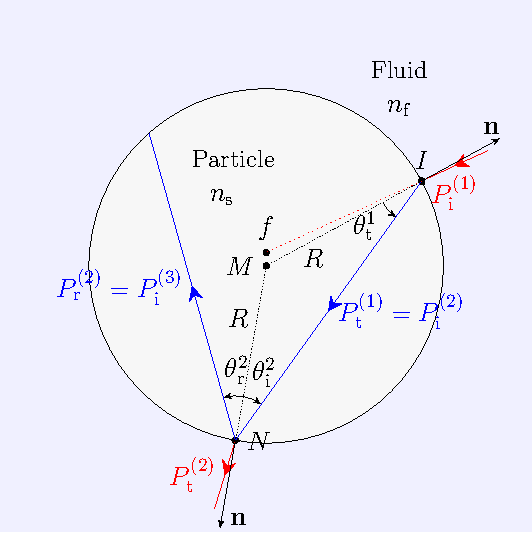
\includegraphics[]{Plots/cache/ray.pdf}
  \caption{Schematic of ray path through particle.}
  \label{fig:Th-ray_particle}
\end{figure}

With the convergence angle $\beta$ (see \cref{fig:Th-angles}) and the sine-law
\begin{equation}
  \frac{\sin\left( \frac{\pi}{2}-\beta \right)}{\R} = 
  \frac{\sin\incident}{a\,\R}
  \label{eq:Th-sine-law}
\end{equation}
one can compute $\incident$ as function of $\beta$. The angle $\beta$ is an 
input parameter and therefore known. The maximal convergence angle 
$\beta_{\MR{max}}$ is evaluated by the definition of the NA
\begin{equation}
  \text{NA} = \nf\,\sin\beta_{\MR{max}}.
  \label{eq:Th-NA}
\end{equation}
Our lens has a NA of 1.27 and water has a refractive index of $\nf=1.33$ (see 
\cref{fig:Th-n_water}) and therefore is our maximal convergence angle 
$\beta_{\MR{max}} \approx \SI{72}{\degree}$.

With the knowledge of $\transmitted^{1}$ the path of the ray inside the 
particle is determined. At the next intersection point of the ray with the 
particle surface $N$, the ray is again partly transmitted into the fluid and 
partly reflected. Since the triangle $\bigtriangleup_{IMN}$ is an isosceles 
triangle (two sides have the same length; here $R$) and per definition the 
reflected angle equals the incident angle, all internal reflection angles for 
one ray have the same magnitude 
($\transmitted^{1}=\incident^{n}=\reflected^{n}$ for $n>1$).

Now, the respective powers of one ray can be evaluated. The ray has the 
incident power $\power{i}{1}$ with every reflection it gets split into two 
portions. With \cref{eq:Th-fresnelR,eq:Th-fresnelT,eq:Th-fresnel} the powers 
after each reflection is
\begin{subequations}
  \begin{alignat}{3}
    \power{t}{1} & = \fresnelT\left( \incident^{1} \right)\,\power{i}{1} && \\
    \power{r}{2} & = \fresnelR\left( \transmitted^{1} \right)\,\power{t}{1} && 
    = \power{i}{1}\,\fresnelT\left( \incident^{1} \right)\,
    \fresnelR\left( \transmitted^{1} \right) \\
    \power{t}{2} & = \fresnelT\left( \transmitted^{1} \right)\,\power{t}{1} && 
    = \power{i}{1}\,\fresnelT\left( \incident^{1} \right)\,
    \fresnelT\left( \transmitted^{1} \right) \\
    \power{r}{3} & = \fresnelR\left( \transmitted^{1} \right)\,\power{i}{3} && 
    = \power{i}{1}\,\fresnelT\left( \incident^{1} \right)\,
    \fresnelR^{2}\left( \transmitted^{1} \right).
\end{alignat}
\end{subequations}

\begin{figure}[thp]
  \centering
  % \tikzsetnextfilename{angles}

\tikzstyle arrowstyle=[scale=2]
\tikzstyle directed=[postaction={decorate,decoration={markings,
    mark=at position .65 with {\arrow[arrowstyle]{stealth}}}}]

\begin{tikzpicture}[scale=1.3]
    \coordinate (O) at (0,0);
    \coordinate (I) at (4,3);
    \coordinate (A) at (0,1.4);

    \node[circle,fill=black,inner sep=0pt,minimum size=3pt,label=below:{$M$}] 
    at (O) {};
    \node[circle,fill=black,inner sep=0pt,minimum size=3pt,label=left:{$f$}] at 
    (A) {};
    \node[circle,fill=black,inner sep=0pt,minimum size=3pt,label=above:{$I$}] 
    at (I) {};

    % \draw (O) -- node[midway, below, xshift=1mm] {$R$} (I) -- node[above, 
    % midway, xshift=-1mm] {$y$} (A) -- node[midway, left] {$a\,R$} cycle;
    \draw (O) -- node[midway, below, xshift=1mm] {$\R$} (I) -- (A) -- 
    node[midway, left] {$a\,\R$} cycle;

    % \draw[dotted] (O) rectangle (I);
    \draw[dotted] (A) -- ++(0,1);

    \draw[->,>=stealth'] (I) -- node[above,midway] {$\normalvector$} (36.86:6);

    \draw[directed,red] (34.0:6.2) -- (I);


    \draw[] (0,0.5) arc (90:37:0.5) node[midway, above] {$\gamma$};
    \draw[] (0,1.9) arc (90:22:0.5) node[midway, above] {$\beta$};
    \draw[] (0,1.1) arc (-90:22:0.3) node[midway, right] 
    {$\sfrac{\pi}{2}-\beta$};
    \draw[] (36.8:3.5) arc (216:200.5:1.5) node[pos=.3, left] {$\incident$};

    \draw[] (I) arc (36.86:48:5);
    \draw[] (I) arc (36.86:-3:5);

\end{tikzpicture}

  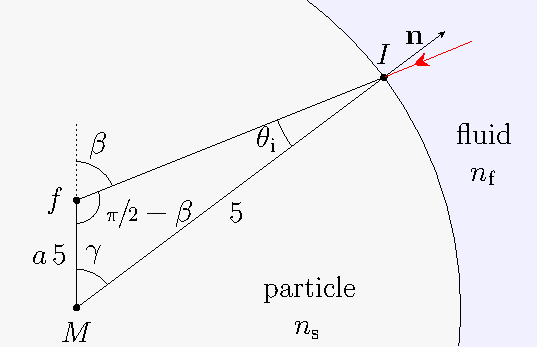
\includegraphics[]{Plots/cache/angles.pdf}
  \caption{Sketch of incident ray onto particle surface.}
  \label{fig:Th-angles}
\end{figure}

If a particle is stably trapped the distance $a$ of the particle center point 
$M$ and the focal point $f$ (see also \cref{fig:Th-angles}) is about $a \approx 
0.1\,R$~\cite{Lamprecht2017}. During the trapping process and due to external 
forces this distances changes. If the focal point is outside the particle, the 
trapping forces are negligible small.

\cref{fig:Th-gamma_theta} depicts the values of $\gamma$ and $\incident$, 
respectively, for different combinations of $a$ and $\beta$. As pointed out 
before, the distance $a$ is about $0.1\,R$. For this value the maximal incident 
angle $\incident$ over the whole range of $\beta$ is less than 
\SI{10}{\degree}.

\begin{figure}
  \centering
  \begin{subfigure}[b]{0.45\textwidth}
    \centering
    % \tikzsetnextfilename{gamma}
%%%%%%%
% READ TABLE
%%%%%%%

\begin{tikzpicture}
    \begin{axis}[view={0}{90},
        xlabel={$a$ [-]},
        ylabel={$\beta$ [\si{\degree}]},
        xmax=0.5,
        height=60mm,
        point meta min=0,
        point meta max=72,
        width=60mm,
        colormap/YlGnBu-9,
        colorbar,
        colorbar horizontal,
        colorbar style={
          title={$\gamma$ [\si{\degree}]},
          at={(0,1.3)},
          anchor=north west,
          xtick={0,24,48,72},
        },
        ytick={0,24,48,72},
        xtick={0,0.25,0.5},
      ]
      % countourf
      \addplot3[surf,mesh/rows=51,shader=interp] table[x=a,y=beta,z=gamma] 
      {\relPath/10_Figures/TikZ/angles_mat.dat};
      % lines
       \addplot3[
         mesh/rows=51,
         mesh/cols=50,
         contour gnuplot={levels={9,18,36,54},draw color=black},
     ] table[x=a,y=beta,z=gamma] {\relPath/10_Figures/TikZ/angles_mat.dat};

    \end{axis}
\end{tikzpicture}

    \caption{}
    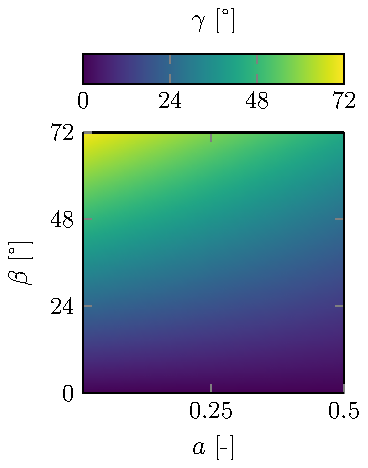
\includegraphics[]{Plots/cache/gamma.pdf}
    \label{fig:Th-gamma}
  \end{subfigure}
  \hfill
  \begin{subfigure}[b]{0.45\textwidth}
    \centering
    % \tikzsetnextfilename{theta_i}
%%%%%%%
% READ TABLE
%%%%%%%

\begin{tikzpicture}
    \begin{axis}[view={0}{90},
        xlabel={$a$ [-]},
        ylabel={$\beta$ [\si{\degree}]},
        xmax=0.5,
        height=60mm,
        point meta min=0,
        point meta max=30,
        width=60mm,
        colormap name=viridis,
        colorbar,
        colorbar horizontal,
        colorbar style={
          title={$\incident$ [\si{\degree}]},
          at={(0,1.3)},
          anchor=north west,
          xtick={0,10,20,30},
        },
        ytick={0,24,48,72},
        xtick={0,0.25,0.5},
      ]
      \addplot3[surf,mesh/rows=51,shader=interp] table[x=a,y=beta,z=theta] 
      {\relPath/10_Figures/TikZ/angles_mat.dat};
    \end{axis}
\end{tikzpicture}

    \caption{}
    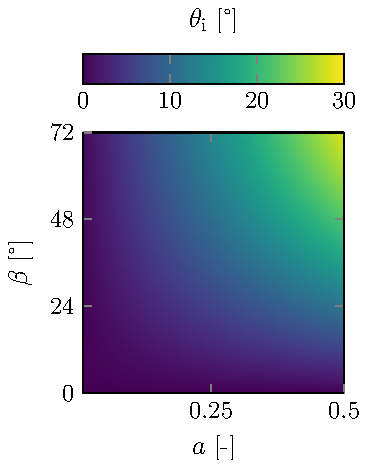
\includegraphics[]{Plots/cache/theta_i.pdf}
    \label{fig:Th-theta_i}
  \end{subfigure}
    \caption{Magnitude of $\gamma$ and $\incident$ for different values of $a$ 
    and $\beta$ (see also \cref{fig:Th-angles}).}
  \label{fig:Th-gamma_theta}
\end{figure}

\begin{figure}[tbp]
  \centering
  % \tikzsetnextfilename{Fresnel}
%%%%%%%
% READ TABLE
%%%%%%%
\pgfplotstableread{\relPath/10_Figures/TikZ/Fresnel.dat}{\data}

\begin{tikzpicture}
  \begin{groupplot}[
    axis on top=true,
    group style={
      group size=2 by 1,
      horizontal sep = 23mm,
    },
    xmin=0,
    ymin=0,
    height=55mm,
    width=73mm,
    no markers,
  ]
  \nextgroupplot[
    xlabel={Incident angle $\incident$ [\si{\degree}]},
    ylabel={\footnotesize Fresnel Coefficient [-]},
    xtick={0,0.16666,0.333333,0.5},
    xticklabels={0, 30, 60, 90},
    legend style={
      at={(axis cs:0.01,0.5)},
      anchor=west,
      font=\footnotesize,
    }
  ]
  \filldraw[black!10!,opacity=0.7] (0.155,0) rectangle ({0.5,1}|-{rel axis 
  cs:1,1});

    \addplot[dashed] table[x=theta,y=R_M2P] {\data};
    \addlegendentry{$\fresnelR_{\mathrm{f\rightarrow s}}$};
    \addplot[] table[x=theta,y=T_M2P] {\data};
    \addlegendentry{$\fresnelT_{\mathrm{f\rightarrow s}}$};

    \addplot[thick, blue, dotted] table[x=theta,y=R_P2M] {\data};
    \addlegendentry{$\fresnelR_{\mathrm{s\rightarrow f}}$};
    \addplot[thick, blue] table[x=theta,y=T_P2M] {\data};
    \addlegendentry{$\fresnelT_{\mathrm{s\rightarrow f}}$};

    \nextgroupplot[
    xlabel={Incident angle $\incident$ [\si{\degree}]},
    xmax=0.167,
    ymin=0.001,
    ymode=log,
    xtick={0,0.05555,0.11111,0.1666666},
    xticklabels={0, 10, 20, 30},
  ]

  \filldraw[black!10!,opacity=0.7] (0.155,0.00001) rectangle ({0.167,1}|-{rel 
  axis cs:1,1});

    \addplot[dashed] table[x=theta,y=R_M2P] {\data};
    \addplot[] table[x=theta,y=T_M2P] {\data};

    \addplot[thick, blue, dotted] table[x=theta,y=R_P2M] {\data};
    \addplot[thick, blue] table[x=theta,y=T_P2M] {\data};

  \end{groupplot}
  % \draw[thick,blue,->,shorten >=2pt,shorten <=2pt] (group c1r1.east) -- (group 
  % c2r1.west);
\end{tikzpicture}

  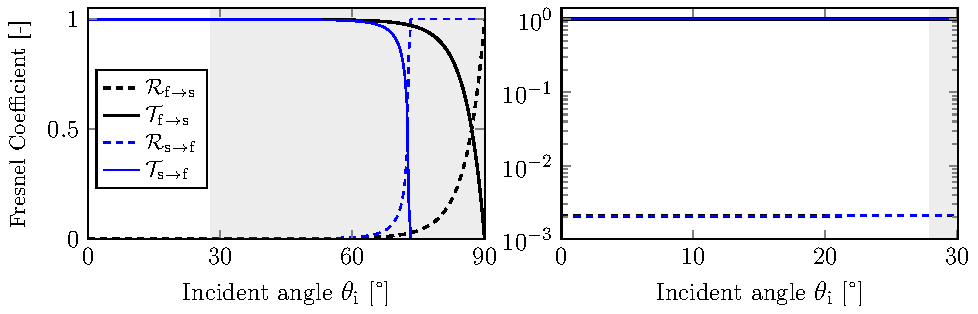
\includegraphics[]{Plots/cache/Fresnel.pdf}
  \caption{Fresnel coefficients of reflectance and transmittance (see 
  \cref{eq:Th-fresnelR,eq:Th-fresnelT}) for a water-particle interface 
  ($\Box_{\MR{f}\rightarrow\MR{s}}$) and a particle-water interface 
($\Box_{\MR{s}\rightarrow\MR{f}}$). The right plot is a detail of the left one 
with a logarithmic y-scale. The grey shaded area marks the interval of incident 
angles $\incident$ that do not occur in our setup.}
  \label{fig:Th-fresnel}
\end{figure}

Finally all is in place, to estimate the total relative absorbed energy 
$\delta$ by the particle.  \cref{eq:Th-intensity} defines the intensity after 
the distance $s$. Hence the relative absorbed energy over this length is
\begin{equation}
    \intensity_{\MR{abs}} = \intensity_{0} \left( 1 - \exp(-\alpha\,s) \right).
    \label{eq:Th-absorbed_energy}
\end{equation}
The distance $s$ for one passage through the particle can be computed as 
function of $\beta$ as
\begin{equation}
  s\left( \beta \right) = 2\,R\,\cos\left( \transmitted\left[ \incident\left( 
    \beta \right) \right]
    \right).
    \label{eq:Th-distance_s}
\end{equation}
And the power of a ray after $j$ reflections is
\begin{equation}
  \power{j}{i} =
  \fresnelT_{\MR{f}\rightarrow\MR{s}}\left( \incident \right) \,
  \fresnelR^{(j-1)}_{\MR{s}\rightarrow\MR{f}}\left( \transmitted \right)
  \label{eq:Th-power}
\end{equation}
With \cref{eq:Th-absorbed_energy,eq:Th-distance_s,eq:Th-power} the relative 
absorbed energy $\delta$ inside the particle can be approximated with discrete 
values
\begin{equation}
  \beta_{n} = \frac{n}{N}\,\beta_{\MR{max}}.
  \label{eq:Th-beta-disc}
\end{equation}
to be
\begin{equation}
  \intensity_{\MR{tot.,abs.}} \approx
  \frac{2\pi}{N}
  \sum\limits_{n=1}^{N}
  \sum\limits_{k=0}^{\infty}\power{i}{k-1}\left( \beta_{n} \right)\left[ 1 - 
  \exp\left( -\alpha\,s\left( \beta_{n} \right) \right) \right]
  \label{eq:Th-total-absorbed}
\end{equation}
where the factor $\sfrac{1}{N}$ is due to the assumption that each ray has the 
same incident power when hitting the particle surface and the factor $2\pi$ for 
considering the full volume of the particle. Per definition is the reflectance 
$\fresnelR$ or the transmittance $\fresnelT$ smaller than 1. This property as 
well as
\begin{equation}
  \sum\limits^{\infty}_{k=0} \Box^{k} = \frac{1}{1-\Box}
  \quad\text{for}\quad\abs{\Box} < 1
\end{equation}
can be applied to \cref{eq:Th-total-absorbed} to simplify the double sum to
\begin{equation}
  \intensity_{\MR{tot.,abs.}} \approx
  \frac{2\pi}{N}
  \sum\limits_{n=1}^{N}
  \fresnelT_{\MR{f}\rightarrow\MR{s}}\left( \incident \right)
  \left[ 1 - \exp\left( -\alpha\,s\left( \beta_{n} \right) \right) \right]
\,\frac{1}{1-\fresnelR_{\MR{s}\rightarrow\MR{f}}\left( \transmitted \right)}
  \label{eq:Th-total-absorbed-simp}
\end{equation}
where $\incident$ and $\transmitted$ are also function of $\beta_{n}$.

\cref{fig:Th-fresnel} depicts the values for $\fresnelT$ and $\fresnelR$ for 
the fluid-particle interface and the particle-fluid interface. Noteworthy is 
the fact, that for the occurring incident angles $\incident \leq 
\SI{10}{\degree}$ the values of $\fresnelR$ for both interface are less than 
$3\cdot 10^{-3}$. Therefore, most of the energy is transmitted and almost none 
reflected. For example, the relative power after one internal reflection and 
for an incident angle of $\incident=\SI{10}{\degree}$ is $\approx 2.07\cdot 
10^{-3}\,\power{i}{1}$ and after two internal reflections already $\approx 
4.31\cdot 10^{-6}\,\power{i}{1}$.

\begin{figure}[tbp]
  \centering
  % \tikzsetnextfilename{absorbed_energies}

\begin{tikzpicture}
  \begin{axis}[
      view={0}{90},
      ylabel={$\nicefrac{\Rprime}{\R}$ [-]},
      xlabel={$R$ [\si{\um}]},
      height=50mm,
      width=100mm,
      point meta min=0.2,
      point meta max=2.7,
      colorbar,
      colormap/BuPu-9,
      colorbar horizontal,
      colorbar style={
        title={\footnotesize Relative absorbed Energy $\Xi$ ($\times 
        10^{-4}$)},
        at={(0,1.4)},
        anchor=north west,
        xtick={0.2,0.5,1.0,1.5,2.0,2.5},
      },
    ]
      % contourf
      \addplot3[surf,mesh/rows=21,shader=interp] table[x=R,y=a,z=alpha] 
      {\relPath/10_Figures/TikZ/absorbed_energies.dat};
      % lines
       \addplot3[
         mesh/rows=21,
         mesh/cols=20,
         contour gnuplot={draw color=black},
     ] table[x=R,y=a,z=alpha] {\relPath/10_Figures/TikZ/absorbed_energies.dat};

  \end{axis}
\end{tikzpicture}

  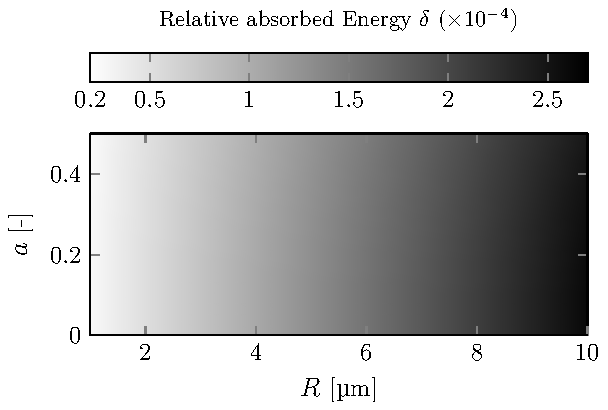
\includegraphics[]{Plots/cache/absorbed_energies.pdf}
  \caption{Results of \cref{eq:Th-total-absorbed-simp} for various relative 
  distances $a$ and radii $R$ with $N=500$ }
  \label{fig:Th-absorbed_energies}
\end{figure}

\cref{fig:Th-absorbed_energies} shows the relative absorbed energy $\delta$ 
inside a particle for various radii $R$ and distances $a\,R$. As 
\cref{fig:Th-fresnel} already suggested only a little fraction of the trapping 
energy is absorbed by the particle itself.

\subsection{Ray Optics Heat Approximation}

\begin{figure}[tbp]
  \centering
  % \tikzsetnextfilename{coordinate}

\begin{tikzpicture}[line cap=round, line join=round, >=Triangle, scale=1.5]

\clip(-2.1,-2.1) rectangle (2.38,2.58);
\filldraw[blue!20,opacity=.3] (-2.1,-2.1) rectangle (2.38,2.58);
\filldraw[white] (0,0) circle (2cm);

\draw[ball color=gray!20!white, fill opacity=0.6] (0,0) circle (2cm);

\draw [rotate around={0.:(0.,0.)},dash pattern=on 3pt off 3pt] (0,0) ellipse 
(2cm and 0.9cm);

\draw (0,0) -- (0.70,1.07) node[right, pos=0.4] {$r$};


\draw[-latex,line width=0.7pt]   (0,0) -- +(0,2) node[above] {$\ez$};
\draw[-latex,line width=0.7pt]   (0,0) -- +(-0.83,-0.81) node [left, 
yshift=-1.8mm] {$\ex$};
\draw[-latex,line width=0.7pt]  (0,0) -- +(2,0) node [right] {$\ey$};


\draw [-Latex, <-, >=stealth', shift={(0,0)}, black, fill opacity=1] (56.7:0.4) 
arc (56.7:90.:0.4) node[above, pos=0.3] {$\theta$};

\begin{scope}[rotate around x=10, y=10, xshift=1, yshift=-4.6]
    \draw [-Latex, ->, >=stealth', shift={(0,0)}, black, fill opacity=1] 
    (-135.7:0.4) arc (-135.7:-33.2:0.4) node[below,pos=0.4] {$\varphi$};
\end{scope}

\draw [dotted] (0.7,1)-- (0.7,-0.46);
\draw [dotted] (0,0)-- (0.7,-0.46);
\draw [fill] (0,0) circle (1.5pt);
\draw [fill] (0.7,1.07) circle (0.5pt);
\end{tikzpicture}

  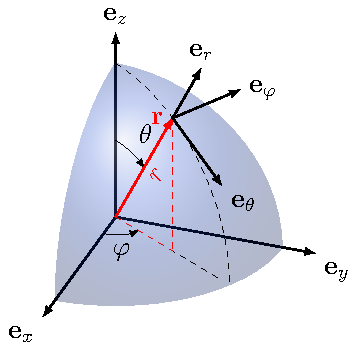
\includegraphics[]{Plots/cache/coordinate.pdf}
  \caption{Sketch of Cartesian and spherical coordinate system}
  \label{fig:Th-coordinate}
\end{figure}

With the knowledge of the relative absorbed energy $\delta$ of the particle, we 
solve the state heat equation for the particle
\begin{equation}
  \laplacian{T} = \frac{1}{\kappa} \pdv{T}{t} - \frac{q}{K}
  \label{eq:Th-heat-prob}
\end{equation}
where $T$ is the temperature inside the particle, $q$ is the absorbed energy of 
unit volume, $K$ the thermal conductivity, and $\kappa$ the thermal 
diffusivity. Further, we neglect the time-dependence $\pdv{T}{t}= 0$
\begin{equation}
  \laplacian{T} = - \frac{q}{K}
  \label{eq:Th-heat-stat}
\end{equation}
because all publications presented in \cref{sec:Th-state} state that the 
heating occurs within \si{\ms} and is negligible afterwards. In addition, we 
assume a spherical particle and solve the problem with spherical coordinate 
system (see \cref{fig:Th-coordinate}) with its origin at the particle center. 
Furthermore, we take the source term $q$ to be constant throughout the 
particle. Therefore, we neglect all partial derivatives to the angles $\varphi$ 
and $\theta$ and solve an ordinary differential equation
\begin{equation}
    \frac{1}{r^{2}}\pdv{r}\left( r^{2}\pdv{T}{r} \right) = - \frac{q}{K}
  \label{eq:Th-heat-spherical}
\end{equation}
with only a $r$ dependence and constant source term. We complete the problem, 
with two boundary conditions
\begin{subequations}
\begin{align}
  \eval{\pdv{T}{r}}_{r=0} &= 0\\[3mm]
  \eval{T}_{r=R_{0}} &= T_{0}.
\end{align}
\end{subequations}
The first one implies a bounded temperature at the origin ($r=0$) and the 
second one fixes the temperature at the surface of the particle ($r=R_{0}$). 
After two consecutive integration and applying of the boundary conditions one 
finds the difference temperature to be
\begin{equation}
  \Delta T(r) = T(r) - T_{0} = \frac{q}{6K}\left( R_0^2 - r^{2} \right).
  \label{eq:Th-heat-sol}
\end{equation}
The average temperature over the whole particle is the volume integral of 
\cref{eq:Th-heat-sol}
\begin{equation}
  \overline{\Delta T} = \frac{1}{V}\int_{V}\Delta T(r) \dd{V} = 
  \frac{1}{15}\,\frac{q}{K}\,R^{2}_{0}.
  \label{eq:Th-heat-avg}
\end{equation}
This can be further simplified since $q$ is the absorbed energy per unit volume
\begin{equation}
  q = \frac{\delta\,P}{V} = \frac{3\delta\,P}{4\,\pi\,R_{0}^{3}}
\end{equation}
where $P$ is the power of the laser and $\delta$ the relative absorbed energy 
of the particle. Finally, the average temperature increase of the spherical 
particle is
\begin{equation}
  \overline{\Delta T} = \frac{1}{20\,\pi}\,\frac{\delta\,P}{R_{0}\,K}.
  \label{eq:Th-heat-sol-simp}
\end{equation}
Interestingly, \cref{eq:Th-heat-sol-simp} seems to scale with $\propto 
\sfrac{1}{R_{0}}$. However, the relative total absorbed energy $\delta$ is also 
dependent on $R_{0}$ because the distance $s$ increases with the particle size 
linearly. But $\delta$ scales with $\left[  1-\exp\left( -\alpha\,R_{0} 
\right)\right]$ and therefore the average difference temperature 
$\overline{\Delta T}$ is proportional to $\sfrac{\left[ 1-\exp\left( 
-\alpha\,R_{0} \right) \right]}{R_{0}}$. This seems counter-intuitive, that 
bigger particle sizes lead to less temperature increase. But this only holds 
for the average temperature difference $\overline{\Delta T}$, the temperature 
distribution $T(r)$ (\cref{eq:Th-heat-sol}) increases with the particle size.

\begin{figure}[tbp]
  \centering
  % \tikzsetnextfilename{dT}
%%%%%%%
% READ TABLE
%%%%%%%
\begin{tikzpicture}
    \begin{axis}[view={0}{90},
        xlabel={$R$ [\si{\um}]},
        ylabel={$P$ [\si{\milli\watt}]},
        height=60mm,
        width=100mm,
        point meta min=0,
        point meta max=70,
        colormap = {whitered}{
          color(0cm) = (white);
          color(1cm) = (red)},
        colorbar,
        colorbar style={
          ytick={0,35,70},
          ylabel={$\overline{\Delta T}$ [\si{\milli\degreeCelsius}]},
        },
        xtick={1,5,10},
      ]
      % contourf
      \addplot3[
        surf,
        mesh/rows=21,
        shader=interp
      ] table[x=R,y=P,z=dT] {\relPath/10_Figures/TikZ/dT.dat};
      % lines
       \addplot3[
         mesh/rows=21,
         mesh/cols=20,
         contour gnuplot={levels={15,30,45,60},draw color=black},
     ] table[x=R,y=P,z=dT] {\relPath/10_Figures/TikZ/dT.dat};
    \end{axis}
\end{tikzpicture}

  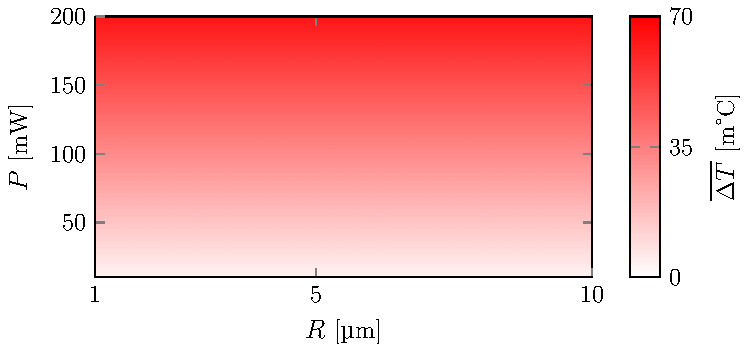
\includegraphics[]{Plots/cache/dT.pdf}
  \caption{$\overline{\Delta T}$ of \cref{eq:Th-heat-sol-simp} for various 
  laser powers $P$ and particle radii $R$.}
  \label{fig:Th-dT}
\end{figure}

\Cref{fig:Th-dT} depicts the average difference temperature for various 
combinations of laser power $P$ and particle radius $R$. With the information 
given in the aforementioned experimental studies regarding the heating by the 
laser and these ray optics motivated results for the heat distribution inside 
the particle, we conclude that the increase in temperature around and inside 
the particle for our setup is less than \SI{2}{\degreeCelsius} with the laser 
power in the low \si{\milli\watt} range we are applying.

Having established an upper bound for the laser induced temperature increase, 
we can estimate the effects of this increase to the absolute value of a 
measured force with the OT. The parameter that changes the most with a change 
in the temperature is the dynamic viscosity $\muef$ of the fluid. The viscosity 
is in general a function of the temperature $\muef\coloneqq\muef(T)$. For our 
calibration routine the absolute measured force of the OT scales with square 
root of the fluid viscosity ($\abs{\vb{\force}}\propto\sqrt{\muef}$). For the 
range of \SIrange{20}{30}{\degreeCelsius} the dynamic viscosity of water (exact 
formula from \cite{Peterman2003}) can be linearly approximated with
\begin{equation}
  \muef(T) = 8.9086\cdot 10^{-4} -2.0277\cdot10^{-5} (T-25).
  \label{eq:Th-viscosity}
\end{equation}
Temperature deviations of $\SI{25}{\degreeCelsius}\pm\SI{2}{\degreeCelsius}$ 
lead to force magnitude errors of less than $\pm$2.5\%.

\section{Optical Position Detection\label{sec:Th-QPD}}

Besides trapping the OT can also measure the relative movement of the trapped 
object within the trap. After a calibration it is also possible to convert the 
movement into the physical unit of meters and then also convert it into a force 
with unit Newton. Besides doing the movement tracking visually with, e.g., a 
high-speed camera, the most common approach is do utilize quadrant photo diodes 
(QPDs). The latter is superior to the camera because higher sampling 
frequencies are straightforward achievable, less data is produced during the 
measurement, as well as, a full three dimensional resolution is at hand.

In order to do so, the laser beam must be collimated after the object trapping 
region and then focussed with separate lenses onto two QPDs (see 
\cref{fig:Th-setup}). While the laser beam is focussed within the aperture of 
the QPD for the in-plane $xy$-direction (QPDxy), the beam is focussed to 
overfill the QPD aperture for the $z$-direction. For all measurements, where 
the measured signal of the QPDs need to be converted to meters, it is crucial 
to operate in the so-called \emph{linear range} of the QPD. In the following, 
we will study what this terms stand for.

A QPD consists of a diode divided into four separate regions. Each of the four 
diodes measures the intensity of light on its respective area and return it as 
voltage. \cref{fig:Th-QPD} is a schematic of the QPDxy where the focussed laser 
spot midpoint $M$ is at $x=x_{0}$ and $y=y_{0}$ and the radius of the laser 
spot is about $\sfrac{1}{5}\,R_{\MR{QPD}}$~\cite{Lamprecht2017}.

The normalized intensity distribution can be defined as
\begin{equation}
  \tilde{\intensity} = \tilde{\intensity}(x, y) = 
  \frac{1}{2\pi\,R_{\MR{spot}}^{2}}\,\exp\left[ 
  -\frac{1}{2}\,\frac{(x-x_{0})^{2} + (y - y_{0})^{2}}{R_{\MR{spot}}^{2}} 
\right]
  \quad \text{with}\quad\int\limits_{\dd{A}}\tilde{\intensity}\dd{A} = 1
    \label{eq:Th-intensity}
\end{equation}
where the radius of the spot is $R_{\MR{spot}}=\sfrac{\RA}{5}$.

\begin{figure}[tbp]
  \centering
  % \tikzsetnextfilename{QPD}
%%%%%%%
% READ TABLE
%%%%%%%

\begin{tikzpicture}

  \coordinate (M) at (-1.5, 0.2);


  \draw[<->,latex-latex] (0, 3.5) -- node[above,pos=0] {$\ey$} (0,0) -- 
  node[above,pos=1] {$\ex$}  (3.5, 0);


  \draw[thick, black] (0,0) circle (3);
  \draw[|latex-{latex}|] (-3, -3.5) -- node[below,midway] {$2\,R_{\MR{QPD}}$} 
  ++(6,0);

  \draw[thick, dotted, black] (-3,0) -- ++(6,0);
  \draw[thick, dotted, black] (0,-3) -- ++(0,6);

  \draw[dotted, thick, red, fill=red!50, opacity=0.3] (M) circle (1);
  \draw[|latex-{latex}|] (-2.5, -1.5) -- node[above,midway] {$\approx 
  \sfrac{2}{5}\,R_{\MR{QPD}}$} ++(2,0);

  \fill (M) circle (0.5mm);
  \node[yshift=3mm,right] at (M) {$M$};
  \draw[thin] (M) -- node[pos=1,right] {\small$y_{0}$} ++(1.5,0);
  \draw[thin] (M) -- node[pos=1,below] {\small$x_{0}$} ++(0,-0.2);


  \foreach \angle [count = \xi] in {60,120,240,300}
  {
    \node at (\angle:2.7) {$V_{\xi}$};
  }

\end{tikzpicture}

  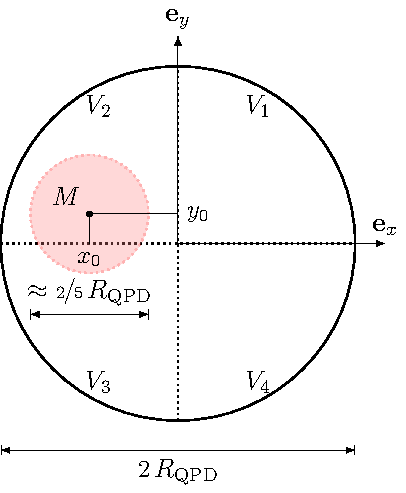
\includegraphics[]{Plots/cache/QPD.pdf}
  \caption{Sketch of quadrant photo detectors for $x$-$y$ detection with center 
  of laser image $M$ at $(x_{0}, y_{0})$.}
  \label{fig:Th-QPD}
\end{figure}

The received intensity $V_{i}$ per quadrant can be evaluated with four 
integrals over the respective areas
\begin{subequations}
\begin{align}
  V_{\MR{1}} & = \int_{0}^{\sfrac{\pi}{2}}\int_{0}^{\RA}
  \tilde{\intensity}\left( r\cos\varphi, r\sin\varphi 
  \right)\,r\,\dd{r}\dd{\varphi}
  \label{eq:Th-V1}
  \\[3mm]
  V_{\MR{2}} & = \int_{\sfrac{\pi}{2}}^{\pi}\int_{0}^{\RA}
  \tilde{\intensity}\left(r\cos\varphi, 
  r\sin\varphi\right)\,r\,\dd{r}\dd{\varphi}
  \label{eq:Th-V2}
  \\[3mm]
  V_{\MR{3}} & = \int_{\pi}^{\sfrac{3\pi}{2}}\int_{0}^{\RA}
  \tilde{\intensity}\left(r\cos\varphi, 
  r\sin\varphi\right)\,r\,\dd{r}\dd{\varphi}
  \label{eq:Th-V3}
  \\[3mm]
  V_{\MR{4}} & = \int_{\sfrac{3\pi}{2}}^{2\pi}\int_{0}^{\RA}
  \tilde{\intensity}\left(r\cos\varphi, 
  r\sin\varphi\right)\,r\,\dd{r}\dd{\varphi}
  \label{eq:Th-V4}
\end{align}
\end{subequations}
where we used polar integration and polar coordinates $x=r\cos\varphi$ and 
$y=r\sin\varphi$.

\begin{figure}[tbp]
  \centering
  % \tikzsetnextfilename{V_quadrant}
%%%%%%%
% READ TABLE
%%%%%%%
\pgfplotstableread{\relPath/10_Figures/TikZ/V_mat.dat}{\data}

\renewcommand{\tikzHelper}{
  \draw[black] (-1,0,0)--(1,0,0);
  \draw[black] (0,-1,0)--(0,1,0);
  \draw[black] (0,0,0) circle (1);
  }

\pgfplotsset{%
    colormap={bwr}{
      color=(blue);
      color=(white);
      color=(red);
    }%
}
%%%%%%%%%%%%%%%%%%%%%%%%%%%%%%%%%%
% Voltages per Quadrant
%%%%%%%%%%%%%%%%%%%%%%%%%%%%%%%%%%

\begin{tikzpicture}
  \begin{groupplot}[view={0}{90},
    % xlabel=$x$,
    % ylabel=$y$,
    height=5cm,
    width=5cm,
    point meta min=0,
    point meta max=1,
    colormap={}{ gray(0cm)=(1); gray(1cm)=(0);},
    group/xlabels at = edge bottom,
    group style = {
      group size = 2 by 2,
      horizontal sep=5mm,
      vertical sep=5mm,
      xlabels at = edge bottom,
      ylabels at = edge bottom
    }]

    \nextgroupplot[
      xticklabels={,,},
      ylabel={$\sfrac{y_{0}}{\RA}$},
    ]
        \addplot3[surf,mesh/rows=99,shader=interp] table[x=x,y=y,z=V4] {\data};
        \tikzHelper

    \nextgroupplot[
      yticklabels={,,},
      xticklabels={,,},
      colorbar right,
      every colorbar/.append style={
        ylabel={Normalized Voltage $\normalized{V}$},
        height=2*\pgfkeysvalueof{/pgfplots/parent axis height}+
        \pgfkeysvalueof{/pgfplots/group/vertical sep}}]
        \addplot3[surf,mesh/rows=99,shader=interp] table[x=x,y=y,z=V1] {\data};
        \tikzHelper

    \nextgroupplot[
      xlabel={$\sfrac{x_{0}}{\RA}$},
      ylabel={$\sfrac{y_{0}}{\RA}$},
    ]
        \addplot3[surf,mesh/rows=99,shader=interp] table[x=x,y=y,z=V3]
        {\data};
        \tikzHelper

    \nextgroupplot[
      xlabel={$\sfrac{x_{0}}{\RA}$},
      yticklabels={,,},
    ]
        \addplot3[surf,mesh/rows=99,shader=interp] table[x=x,y=y,z=V2] {\data};
        \tikzHelper


  \end{groupplot}
\end{tikzpicture}

  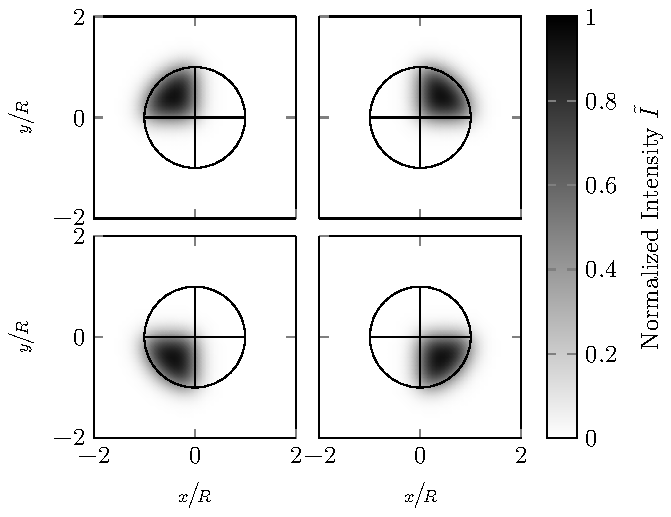
\includegraphics[]{Plots/cache/V_quadrant.pdf}
  \caption{Intensity per quadrant for various positions of laser image middle 
    point $M$ (see \cref{eq:Th-V1,eq:Th-V2,eq:Th-V3,eq:Th-V4}). The top right 
  plot is $V_{1}$, top left $V_{2}$, bottom left $V_{3}$, bottom right 
$V_{4}$.}
  \label{fig:Th-quadrant_Intensity}
\end{figure}

If the particle moves within the trap the center of the laser image $M$ on the 
QPDxy also moves. \cref{fig:Th-quadrant_Intensity} shows the intensity per 
quadrant for different center positions. As expected, each quadrant is 
measuring the highest intensity whenever most of the laser image is over the 
respective area.

With these for separate values for $V_{1}$ through $V_{4}$, one can create a 
measure that is proportional to the movement of the laser image center $M$ 
along the $\ex$- and $\ey$-direction, respectively. The measure is a addition 
and subtraction of the quadrants along one direction
\begin{subequations}
\begin{align}
  V_{\MR{x}} & = \left( V_{\MR{1}}+V_{\MR{4}} \right) - \left( V_{\MR{2}} + 
  V_{\MR{3}}  \right)
  \label{eq:Th-Vx} \\
  V_{\MR{y}} & = \left( V_{\MR{1}}+V_{\MR{2}} \right) - \left( V_{\MR{3}} + 
  V_{\MR{4}}  \right)
  \label{eq:Th-Vy} \\
  V_{\MR{t}} & = V_{\MR{1}}+V_{\MR{2}} + V_{\MR{3}} + V_{\MR{4}}.
  \label{eq:Th-Vt}
\end{align}
\end{subequations}

 \begin{figure}
  \centering
  \begin{subfigure}[b]{0.35\textwidth}
    \centering
    % \caption{$V_{\MR{x}}$}
    % \tikzsetnextfilename{QPDx}

\renewcommand{\tikzHelper}{
  \draw[black] (-1,0,0)--(1,0,0);
  \draw[black] (0,-1,0)--(0,1,0);
  \draw[black] (0,0,0) circle (1);

  \draw[black, dotted] (-1.5,0,0) -- (1.5,0,0);
  \draw[black, dotted] (-1.5,-0.6,0) -- (1.5,-0.6,0);
  \draw[black, dotted] (-1.5,0.6,0) -- (1.5,0.6,0);
}

\begin{tikzpicture}
  \begin{axis}[view={0}{90},
      xlabel=$\sfrac{x_{0}}{\RA}$,
      ylabel=$\sfrac{y_{0}}{\RA}$,
      point meta min=-1,
      point meta max=1,
      height=48mm,
      width=48mm,
      colormap/PuOr-11,
      colorbar,
      colorbar horizontal,
      colorbar style={
        title={\footnotesize Normalized Voltage $\normalized{V}_{x}$},
        at={(0,1.4)},
        anchor=north west,
        xtick={-1,0,1},
      }
    ]
      \addplot3[surf,mesh/rows=99,shader=interp] table[x=x,y=y,z=Vy] 
      {\relPath/10_Figures/TikZ/V_mat.dat};
    \tikzHelper
  \end{axis}
\end{tikzpicture}

    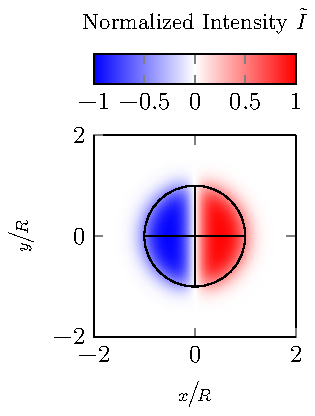
\includegraphics[]{Plots/cache/QPDx.pdf}
    \label{fig:Th-QPDx}
  \end{subfigure}
  \hfill
  \begin{subfigure}[b]{0.3\textwidth}
    \centering
    % \caption{$V_{\MR{y}}$}
    % \tikzsetnextfilename{QPDy}

\renewcommand{\tikzHelper}{
  \draw[black] (-1,0,0)--(1,0,0);
  \draw[black] (0,-1,0)--(0,1,0);
  \draw[black] (0,0,0) circle (1);
}

\pgfplotsset{%
    colormap={bwr}{
      color=(blue);
      color=(white);
      color=(red);
    }%
}

\begin{tikzpicture}
  \begin{axis}[view={0}{90},
      xlabel=$\sfrac{x}{\R}$,
      yticklabels={,,},
      point meta min=-1,
      point meta max=1,
      height=50mm,
      width=50mm,
      colorbar,
      colorbar horizontal,
      colorbar style={
        title={\footnotesize Normalized Intensity $\normalized{\intensity}$},
        at={(0,1.4)},
        anchor=north west,
        xtick={-1,-0.5,...,1},
      }
    ]
      \addplot3[surf,mesh/rows=51,shader=interp] table[x=x,y=y,z=Vx] 
      {\relPath/10_Figures/TikZ/V_mat.dat};
    \tikzHelper
  \end{axis}
\end{tikzpicture}

    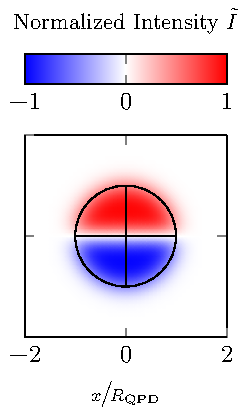
\includegraphics[]{Plots/cache/QPDy.pdf}
    \label{fig:Th-QPDy}
  \end{subfigure}
  \hfill
  \begin{subfigure}[b]{0.3\textwidth}
    \centering
    % \caption{$V_{\MR{t}}$}
    % \tikzsetnextfilename{QPDt}

\begin{tikzpicture}
  \begin{axis}[view={0}{90},
      xlabel=$\sfrac{x_{0}}{\RA}$,
      yticklabels={,,},
      height=48mm,
      width=48mm,
      colormap name=WhiteOr,
      colorbar,
      colorbar horizontal,
      colorbar style={
        title={\footnotesize Normalized Voltage $\normalized{V}_{t}$},
        at={(0,1.4)},
        anchor=north west,
        xtick={0,0.5,1},
      }
    ]
      \addplot3[surf,mesh/rows=99,shader=interp] table[x=x,y=y,z=V] 
      {\relPath/10_Figures/TikZ/V_mat.dat};

  \draw[black] (-1,0,0)--(1,0,0);
  \draw[black] (0,-1,0)--(0,1,0);
  \draw[black] (0,0,0) circle (1);

  \draw[black, dotted] (-1.5,0,0) -- (1.5,0,0);
  \draw[black, dotted] (-1.5,-0.6,0) -- (1.5,-0.6,0);
  \draw[black, dotted] (-1.5,0.6,0) -- (1.5,0.6,0);
  \end{axis}
\end{tikzpicture}

    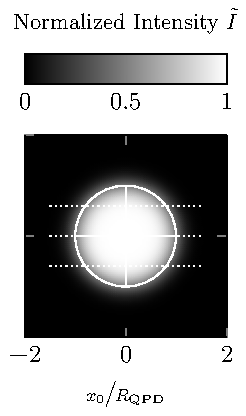
\includegraphics[]{Plots/cache/QPDt.pdf}
    \label{fig:Th-QPDt}
  \end{subfigure}
  \caption{QPD measure $V_{\MR{x}}$ (left;~\cref{eq:Th-Vx}), $V_{\MR{y}}$ 
    (center;~\cref{eq:Th-Vy}), and $V_{\MR{t}}$ (right;~\cref{eq:Th-Vt}) for 
    various positions of laser image middle point $M$. The dotted horizontal 
    lines are at $y=\sfrac{-0.6}{R_{\MR{QPD}}}$, $y=\sfrac{0}{R_{\MR{QPD}}}$, 
  and $y=\sfrac{0.6}{R_{\MR{QPD}}}$ respectively.}
  \label{fig:Th-QPDs}
 \end{figure}

As for the measured intensity per quadrant, the measured values are highest if 
the laser image is over the respective quadrants (see \cref{fig:Th-QPDs}). 
However, since $V_{\MR{x}}$ and $V_{\MR{y}}$ are composed by addition and 
subtraction of the strictly positive values $V_{i}$ the magnitude can now also 
be negative.

In \cref{fig:Th-voltages_over_x} the three measures are plotted over $x_{0}$ 
for three fixed values of $y_{0}$. This plot looks the same if $x_{0}$ is fixed 
and $y_{0}$ is the changing variable. Additionally the curves $V_{\MR{x}}$ and 
$V_{\MR{y}}$ change their behavior. It is clear, that there is a linear region 
for which a little movement of the laser image middle point $M$ is converted 
into a proportional change in the measured intensity on the QPD. However, this 
\emph{linear regime} from $-0.15\,R_{\MR{QPD}}$ to $0.15\,R_{\MR{QPD}}$ is 
rather little. Therefore, it is very important to check and adjust the offset 
of the QPD before each measurement to ensure interpretability of the results.

Noteworthy is also that for values of $\sfrac{\abs{x_{0}}}{R_{\MR{QPD}}} > 0.5$ 
a further outwards movement does not lead to an increase of the respective 
measure but to a decrease. If just one measure, here $V_{\MR{y}}$, is taken 
into account then this decrease ($\sfrac{x_{0}}{R_{\MR{QPD}} > 0.5}$) is not 
distinguishable from the increase coming from the middle 
($\sfrac{x_{0}}{R_{\MR{QPD}} < 0.5}$). However, by also looking at the 
evolution of $V_{\MR{t}}$ it is possible to identify in which direction the 
laser image is moving on the QPD because this measure does not change its 
magnitude between $\sfrac{\abs{x_{0}}}{R_{\MR{QPD}}} < 0.5$.

\begin{figure}[tbp]
  \centering
  % \tikzsetnextfilename{voltages_over_x}
%%%%%%%
% READ TABLE
%%%%%%%
\pgfplotstableread{\relPath/10_Figures/TikZ/V_line.dat}{\data}

\renewcommand{\tikzHelper}{
  \filldraw[black!10!, opacity=0.5] (-1,-1.1) rectangle (1,1.1);
}

\begin{tikzpicture}
\begin{groupplot}[
    group style={
        group name=myplot,
        group size= 1 by 3,
        vertical sep=8mm,
        },
    height=40mm,
    width=120mm,
    ymin=-1.1,
    ymax=1.1,
    ]
    \nextgroupplot[
    % ylabel={$\tilde{I}$},
      xticklabels={,,},
      title={$y = \sfrac{-0.64}{\RA}$},
      title style={yshift=-2mm},
      ]
      \tikzHelper
      \addplot[dotted] table[x=x,y=Vx_1] {\data};
      \addlegendentry{$V_{\MR{x}}$};
      \addplot[] table[x=x,y=Vy_1] {\data};
      \addlegendentry{$V_{\MR{y}}$};
      \addplot[dashed] table[x=x,y=V_1] {\data};
      \addlegendentry{$V_{\MR{t}}$};
    \nextgroupplot[
      % ylabel={$\tilde{I}$},
      title={$y = \sfrac{0}{\RA}$},
      title style={yshift=-2mm},
      xticklabels={,,},
      ylabel={Normalized Intensity $\normalized{\intensity}$},
      every axis y label/.append style={at=(ticklabel cs:0.5)}
      ]
      \tikzHelper
      \addplot[dotted] table[x=x,y=Vx_2] {\data};
      \addplot[] table[x=x,y=Vy_2] {\data};
      \addplot[dashed] table[x=x,y=V_2] {\data};
    \nextgroupplot[
      % ylabel={$\tilde{I}$},
      xlabel={$\sfrac{x}{\RA}$},
      title={$y = \sfrac{0.64}{\RA}$},
      title style={yshift=-2mm},
      ]
      \tikzHelper
      \addplot[dotted] table[x=x,y=Vx_3] {\data};
      \addplot[] table[x=x,y=Vy_3] {\data};
      \addplot[dashed] table[x=x,y=V_3] {\data};
\end{groupplot}
\end{tikzpicture}

  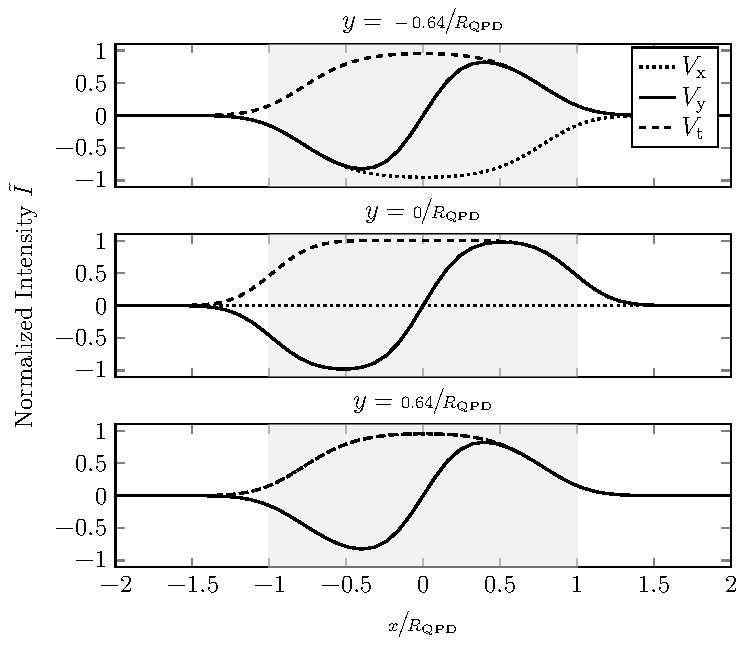
\includegraphics[]{Plots/cache/voltages_over_x.pdf}
  \caption{QPD measure $V_{\MR{x}}$ (\cref{eq:Th-Vx}), $V_{\MR{y}}$
    (\cref{eq:Th-Vy}), and $V_{\MR{t}}$ (\cref{eq:Th-Vt}) over $x_{0}$ for 
  three fixed values of $y_{0}$. The light shaded gray area marks the 
boundaries of the QPD and the dark shaded gray area the linear region of the 
QPD from $-0.15\,R_{\MR{QPD}}$ to $0.15\,R_{\MR{QPD}}$.}
  \label{fig:Th-voltages_over_x}
\end{figure}
